\chapter{Implementation}

\section{System Architecture}
\label{sec:sys-arch}

\begin{figure}[H]
    \centering
    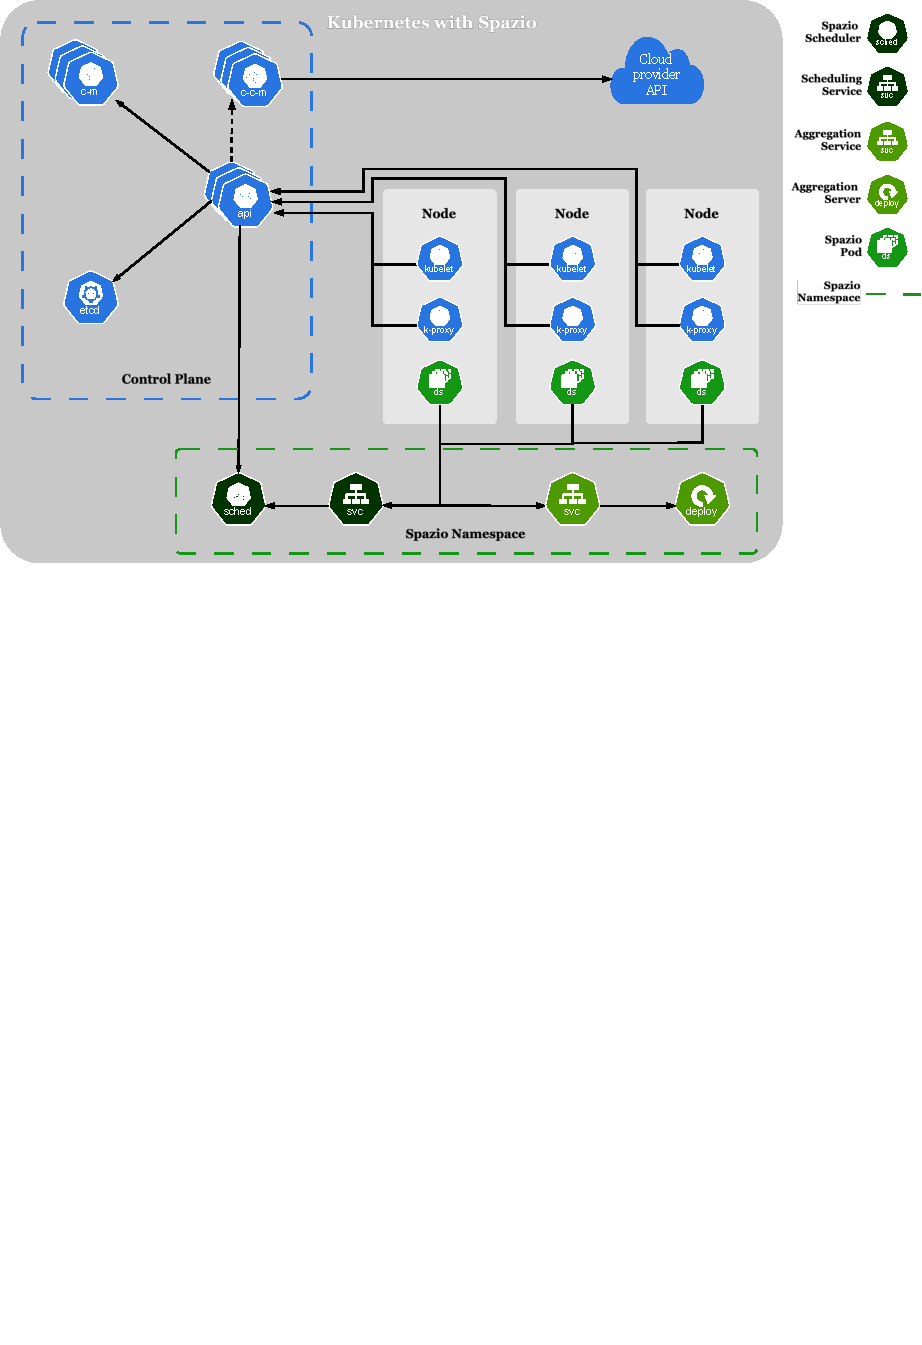
\includegraphics[width=\textwidth]{images/spazio-svg.pdf}
    \caption{The components within the Spazio system}
    \label{fig:spazio-system}
\end{figure}

The Spazio system consists of three core components (shown in figure
\ref{fig:spazio-system}):
\begin{itemize}
    \item Spazio DaemonSet: each Node in the cluster will contain a Spazio Pod.
        This pod periodically collects telemetry from the Node and generates its
        local model and a capacity signal, which it sends to the Scheduling
        Service. When the Spazio Pod deems its local model outdated, it requests
        the latest aggregated global model from the Aggregation service.
    \item Scheduler: In Spazio, the scheduler is a \textbf{Scheduler Plugin},
        implementing custom Filter, Score and Reserve functions. It also acts as
        the server of the Scheduling service, receiving the latest capacity
        scores of each Node to inform its scheduling decisions.
    \item Aggregation Server: This deployment provides the Aggregation service.
        The Aggregation Server Pod receives local models from Nodes
        and returns the latest aggregated global model.
\end{itemize}

\section{Spazio Pod}
\begin{figure}[H]
    \centering
    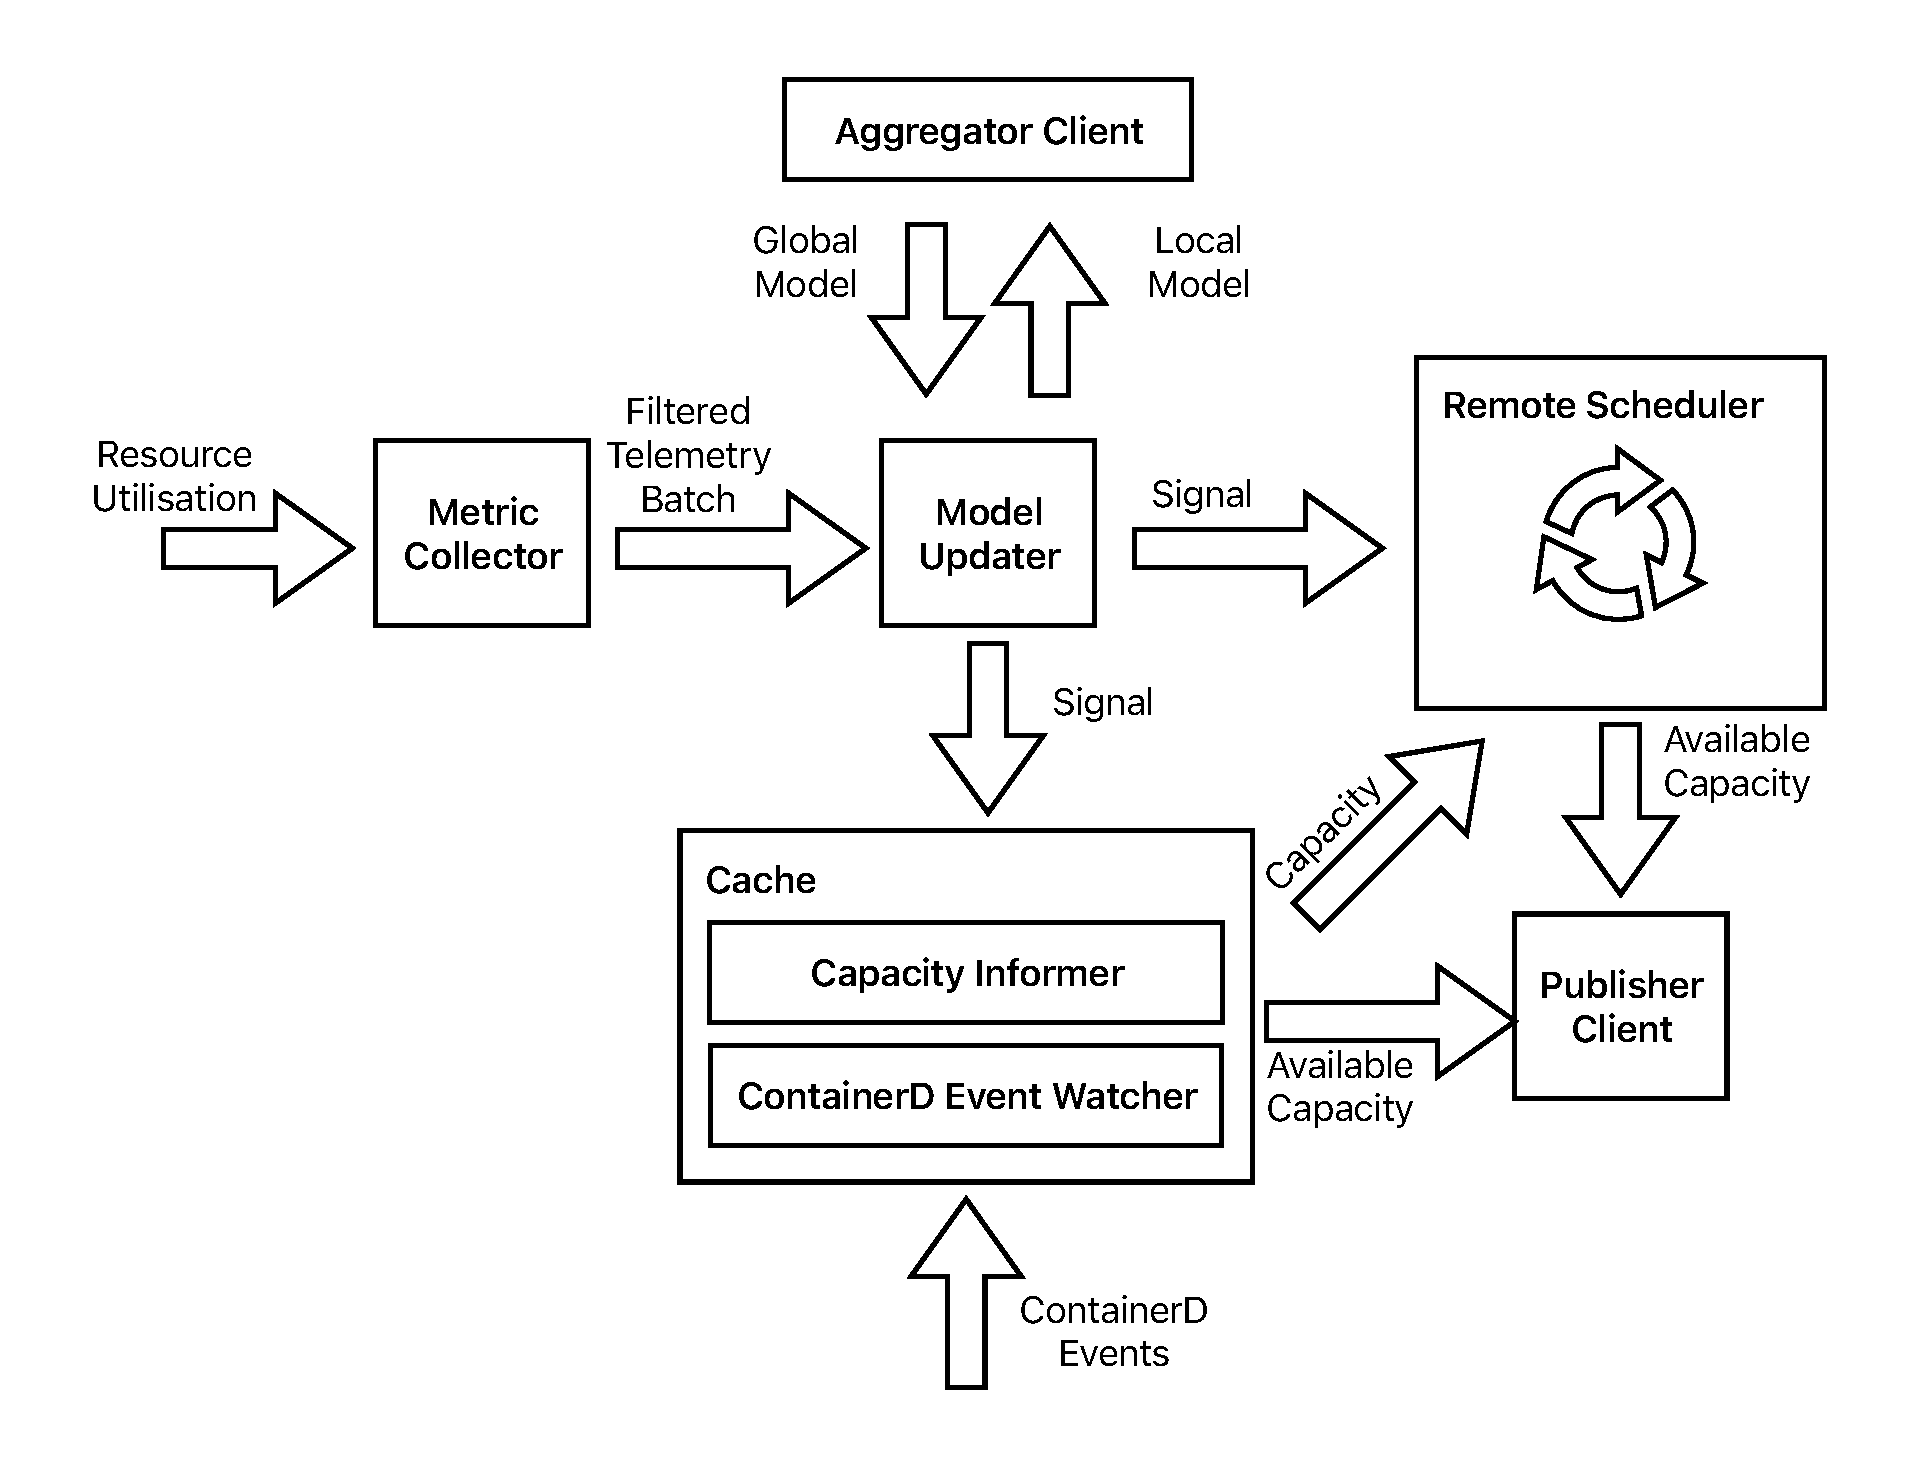
\includegraphics[width=\textwidth]{images/spazio-pod.pdf}
    \caption{Core components within the Spazio pod}
    \label{spazio-pod-components}
\end{figure}
As mentioned in section \ref{sec:sys-arch}, the Spazio Pods are defined within a
DaemonSet - a DaemonSet ensures that all Nodes run a copy of a Pod. The Spazio
Pods collect telemetry from the Node and generate its local model and capacity
signal. The following sections will delve deeper into the implementation
decisions behind the Spazio Pods.

\subsection{Metric Collection}
To build its local model, the Spazio Pod must first collect telemetry. In
Kubernetes there are numerous ways to obtain telemetry data. During my project,
I explored two sources of telemetry data:
\begin{itemize}
    \item Metrics Server: a cluster add-on that acts as a centralised source of
        container reosurce metrics.
    \item \verb|/proc/|: a pseudo-filesystem within Linux that exposes real0time
        information about running processes and system's hardware.
\end{itemize}

With Metrics Server, a scraper is used to periodically (default every 15
seconds) collects resource metrics from Kubelets and exposes them from its
\verb|metrics.k8s.io/v1| APIService. While it is simple to use, it
provides a limited range of metrics, only CPU and RAM utilisation, and
introduces another layer of latency. Furthermore, 15 seconds between scraping is
too long as Pods may complete in under 15 seconds, and therefore, risk not being
detected at all.

TODO: INCLUDE POINT THAT LOCAL MODEL TAKES $B$ SAMPLES AND THEREFORE INCREASES
LATENCY.

On the other hand, \verb|/proc/| can be read from with very little latency,
providing the most up-to-date view of the current state of the system.
Furthermore, \verb|/proc/| contains various files and subdirectories, each
providing specific information. Examples include, \verb|/proc/stat| which
contains the amount of time CPU cores spend in different states,
\verb|/proc/meminfo| provides statistics about memory usage,
\verb|/proc/diskstats| presents the raw, low-level I/O statistics of all block
devices. Finally, the metrics are not generated periodically, but rather
on-the-fly. This guarantees that the information you see is as current as the
system's internal state.

Due to the overwhelming benefits, I decided to use \verb|/proc/| as the source
of my telemetry data. The following sections the different metrics I considered,
providing explainations to implementation decisions.

% I decided to collect CPU and memory utilisation as my telemetry data, as these
% metrics are easily accessible and are used in a variety of industry-standard
% schedulers
 % In addition, it would take $15 \times \text{batch size}$
% seconds between model updates (required to collect a single
% batch before performing subspace merging), and would result in a less
% representative and out-of-date model of "current" resource usage.

\subsubsection{Utilisation Metrics}
Utilisation metrics, such as \% CPU utilised or \% Memory available, are
de-facto metrics when implementing industry-standard
\cite{hadoop2016apache,sahasrabudhe_improved_2015}. These metrics can also be
collected from \verb|/proc/|.

To collect CPU utilisation, I used the \verb|/proc/stat| file. This file reports
the cumulative count of "jiffies" (typically hundredths of a second) each CPU
spent in a specific mode \cite{proc_stat5}. I can then calculate CPU utilisation
using:
\[ \text{CPU Usage\%} = 1 - \frac{\Delta\text{idle} +
\Delta\text{iowait}}{\Delta\text{across all fields}} \]
\verb|/proc/meminfo| can also be used to collect memory utilisations. This file
shows a snapshot of the memory usage in kilobytes. The percentage of memory
used can then be calculated from the given field:
\[ \text{Memory Used\%} = 1 - \frac{\text{MemFree} +
\text{Buffers} + \text{Cached}}{\text{MemTotal}}\]

\begin{figure}[H]
    \centering
    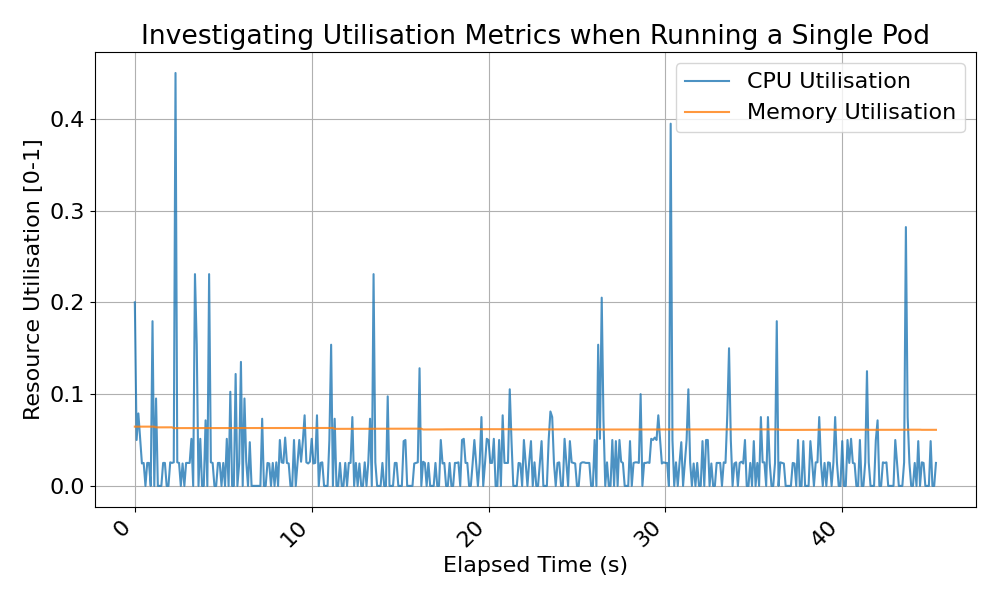
\includegraphics[width=0.45\textwidth]{images/utilisation-baseline.png}
    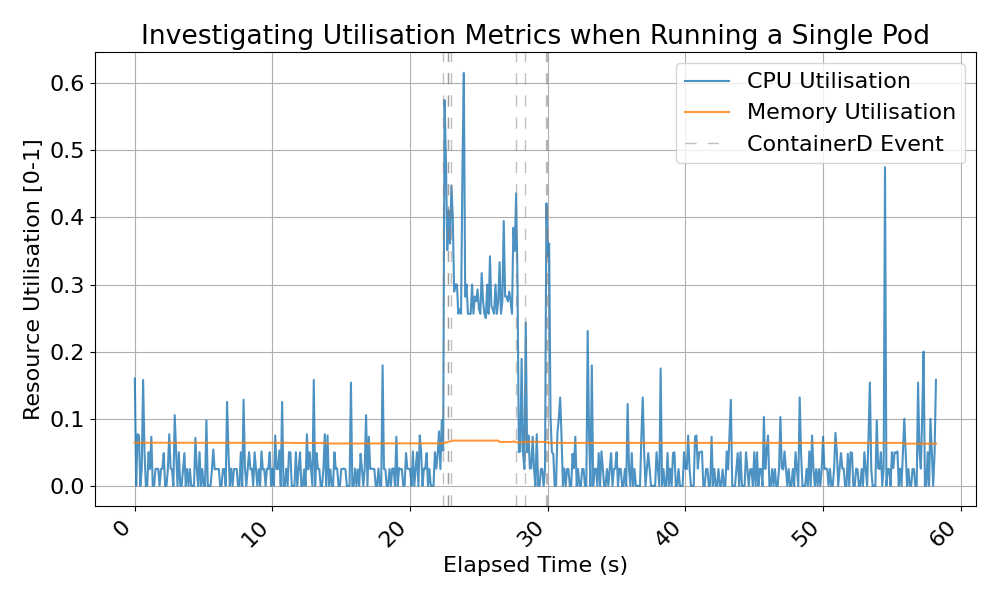
\includegraphics[width=0.45\textwidth]{images/utilisation-single.png} \\
    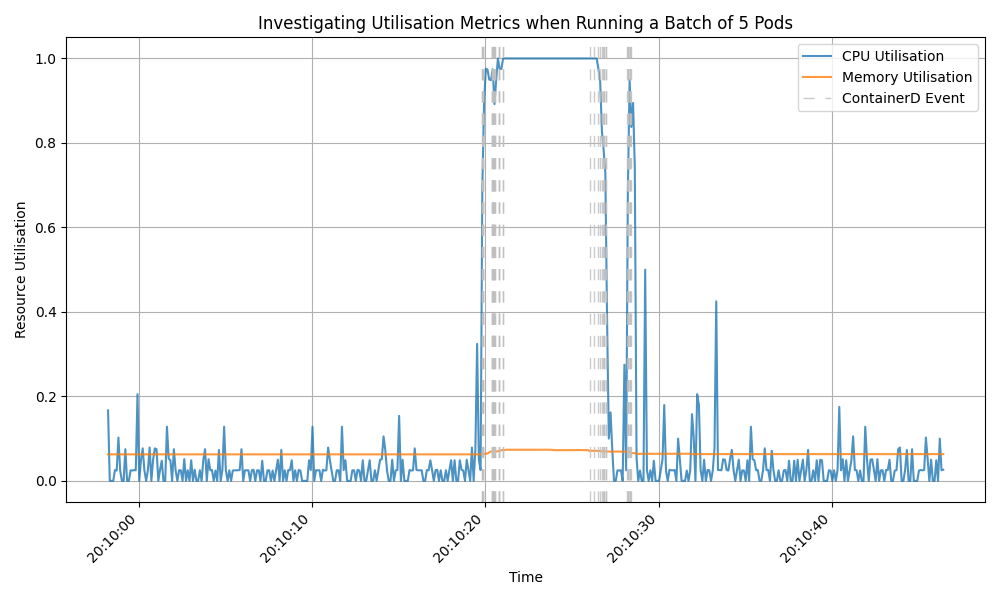
\includegraphics[width=0.45\textwidth]{images/utilisation-smallbatch.png}
    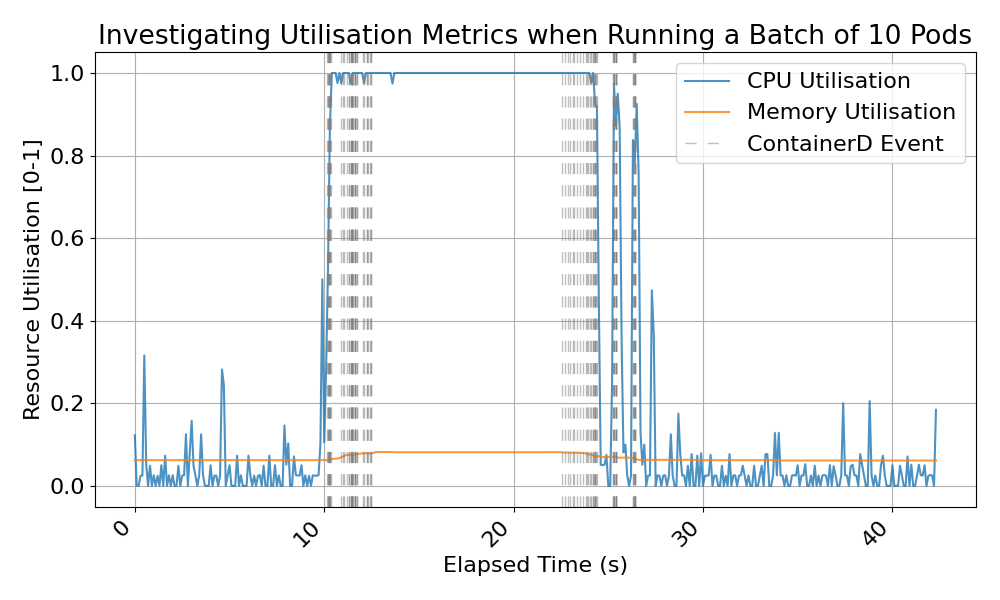
\includegraphics[width=0.45\textwidth]{images/utilisation-bigbatch.png}
    \caption{In this figure we sample CPU and memory utilisation from
    values of \texttt{/proc/stat}, \texttt{/proc/meminfo} at 10Hz during various Kubernetes workload.}
    \label{fig:utilisation-eval}
\end{figure}

To evaluate whether utilisation metrics were suitable for Spazio, I measured
their output under different different workloads. Figure
\ref{fig:utilisation-eval} presents the metrics behaviour when running different
Job sizes of \verb|pi-2000| Pods. As the cpu-intense workload involves
calculating $\pi$ to 2000 digits, we can see how the CPU utilisation correctly
increases for that node while memory utilisation remains constant.

\subsubsection{Issues of using CPU Utilisation}
While evaluating early versions of the prototype which only used utilisation
metrics, its lackluster throughput compared to the default \verb|kube-scheduler|
illuminated a problem of CPU utilisation. When deploying 1000 Pods, each
requesting 100 milliseconds of CPU time, across 19 Nodes, the
\verb|kube-scheduler| would immediately allocate all pods evenly across the
Nodes. This would result in $\approx$ 45 pods running on each node. Meanwhile,
Spazio with only utilisation telemetry would allocate at most 5 Pods at once on
a Node. In both situations, CPU utilisation was 100\%, however, the default
\verb|kube-scheduler| managed to achieve a high throughput with a long-tailed
distribution of individual Pod completion times.

\begin{figure}[H]
    \centering
    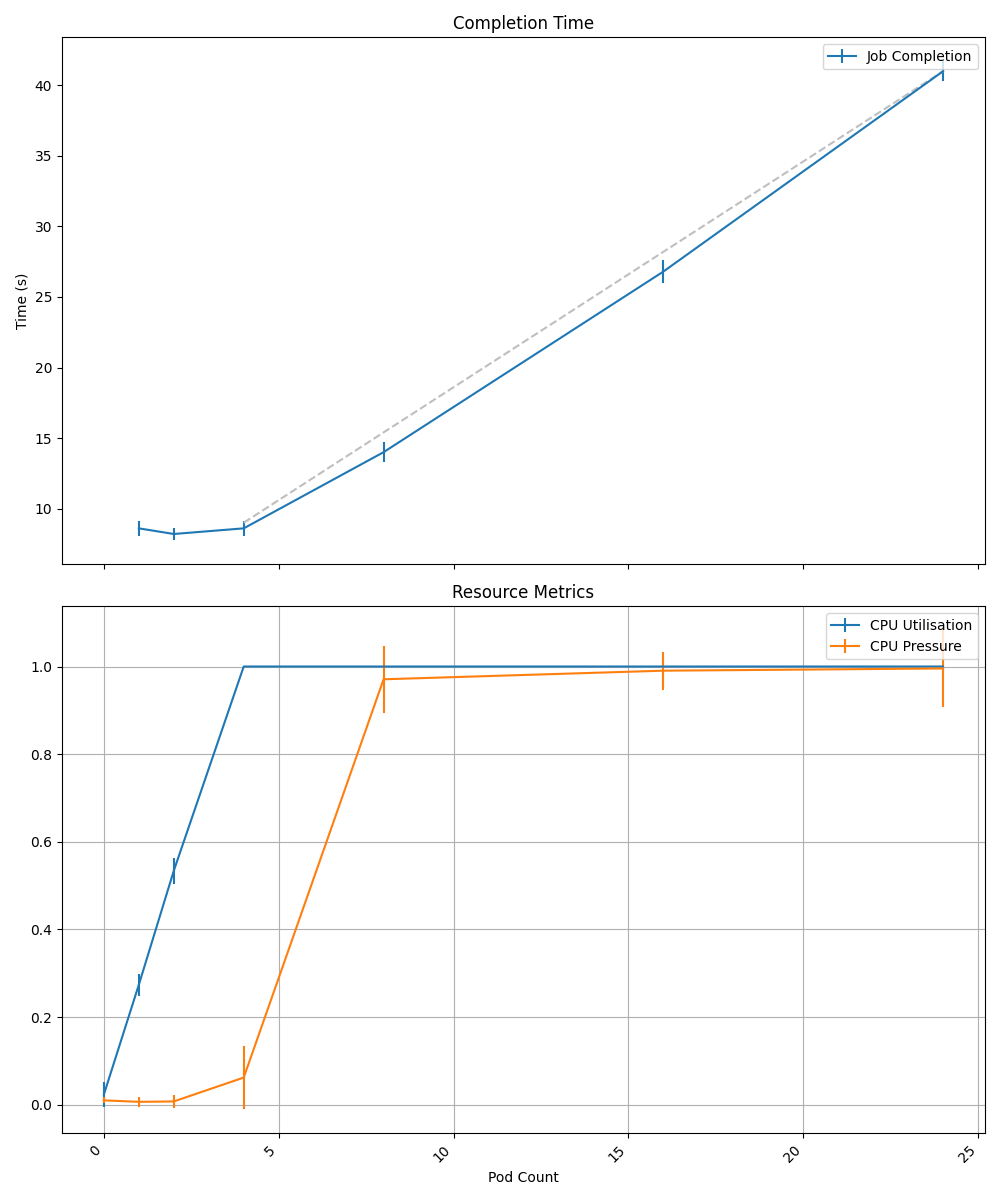
\includegraphics[width=0.45\textwidth]{images/podcount-util-pressure.png}
    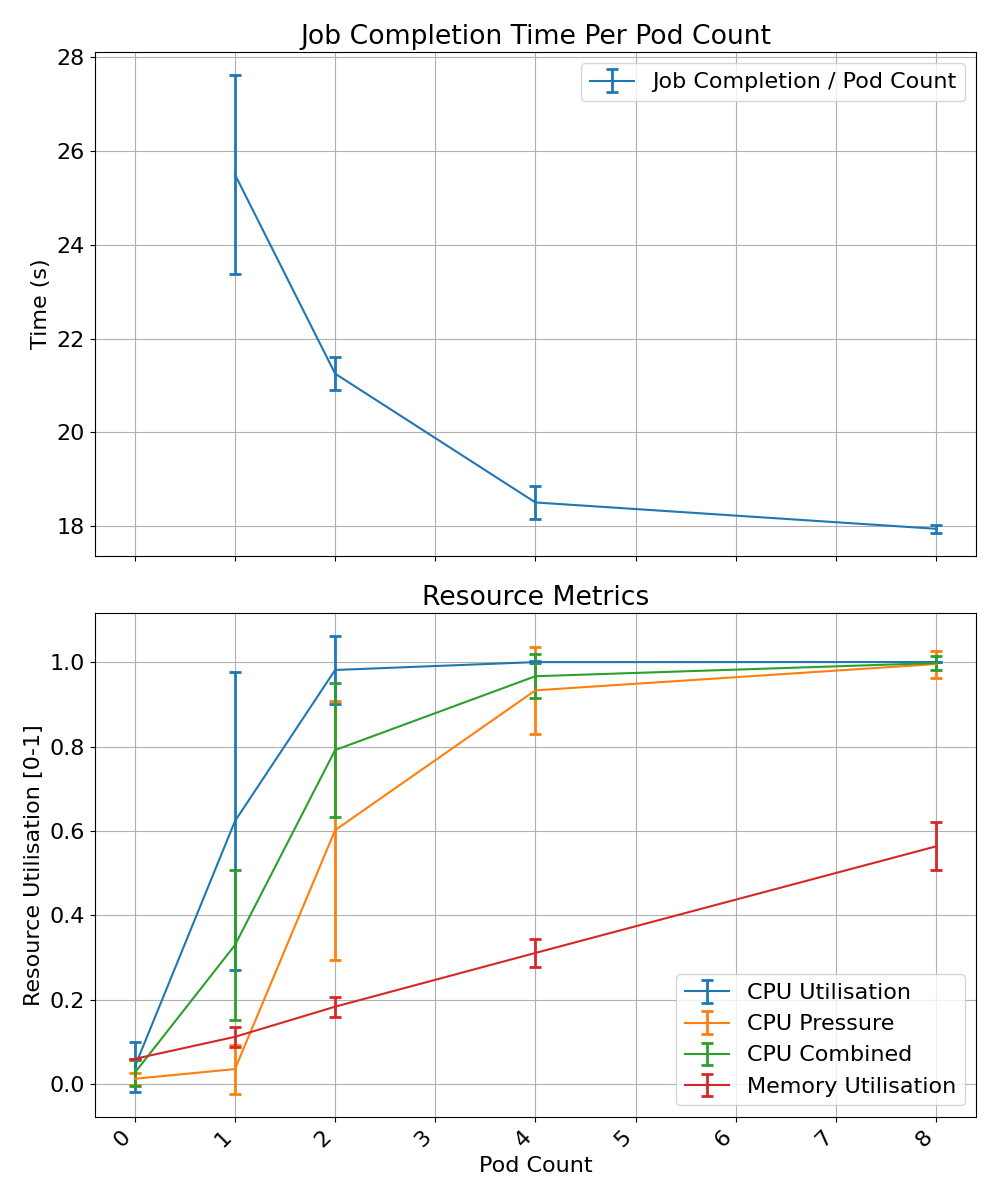
\includegraphics[width=0.45\textwidth]{images/ml-podcount-util-pressure.png}
    \caption{In this figure we sample CPU and memory utilisation from
    values of \texttt{/proc/stat}, \texttt{/proc/meminfo} at 10Hz during various Kubernetes workload.}
    \label{fig:podcount-util-pressure}
\end{figure}

As a result, I decided to further investigate this phenomenon. Figure
\ref{fig:podcount-util-pressure} shows how a Job's completion time changes as you
increase its completion and parallelism count when running different Pods:
cpu-intense Pi-2000 and a small ML workload (training and inference). I also
decided to include measurements from \verb|/proc/pressure|. This investigation
revealed that the relationship between the number of pods running on
a node at a time and their completion time showed a close-to linear
relationship. I hypothesise that this is caused by the cluster being run on top
of VMs. As hypervisors aim to abstract the underlying hardware from the VMs, it
also inadvertently hides hardware effects, such as cache contention and CPU
thrashing. This means that high  CPU utilisation may not truly signify
performance degradation. Therefore, CPU utilisation is not a definitive measure
of resource capacity, and explains why older versions of the  prototype were not
able to push through in terms of pod count and achieve higher throughput.

\subsubsection{Combining CPU Utilisation and CPU Pressure}
Using raw \verb|/proc/pressure| metrics would also not suffice as these metrics
barely increase until the pod count pushes past the number of cores. Therefore,
the intial per-Pod costs for the first few Pods would be unreasonably low and
would result in a Node advertising a falsely high Pod capacity. I instead chose
to combine both CPU utilisation and CPU pressure into a single metric using:
\[ CPU = \frac{\text{CPU Utilisation} + \text{CPU Pressure}}{2} \]

This ensures the metric steadily increases with the number of Pods running on a
Node, but prevents the CPU metric from reaching $1$ to quickly. Instead, the CPU
metric is only maximised once \verb|/proc/pressure| measures that there was
always at least one thread waiting for the CPU.

\begin{figure}[H]
    \centering
    
\includegraphics[width=0.45\textwidth]{images/blank.pdf}
    \caption{In this figure we investigate the behaviour of combining both CPU
    Utilisation and CPU Pressure.}
    \label{fig:combine-cpu-pressure}
\end{figure}

\subsection{Filtering Metrics}
While Spazio doesn't perform peak detection, the signal will still be influenced
by short-lived spikes. As mentioned in the earlier section, pod creation and
deletion incurs a visible spike in resource usage. This spike introduces noise
into a Node's local model, as well as, its capacity signal. A noisy signal can
also make it difficult to achieve accurate capacity and per-Pod cost estimation.
As such, I needed to de-noise the original metrics.

Investigation into the recorded telemetry showed that the spikes caused from
container events would last $\approx$200 milliseconds. Thus when sampling at a
10Hz frequency we can use Dynamic EMA to suppress container-event caused spikes
but allow the smoothed metric to quickly converge on the new utilisation if the
spike exceeded the 300 millisecond threshold.

\begin{figure}[H]
    \centering
    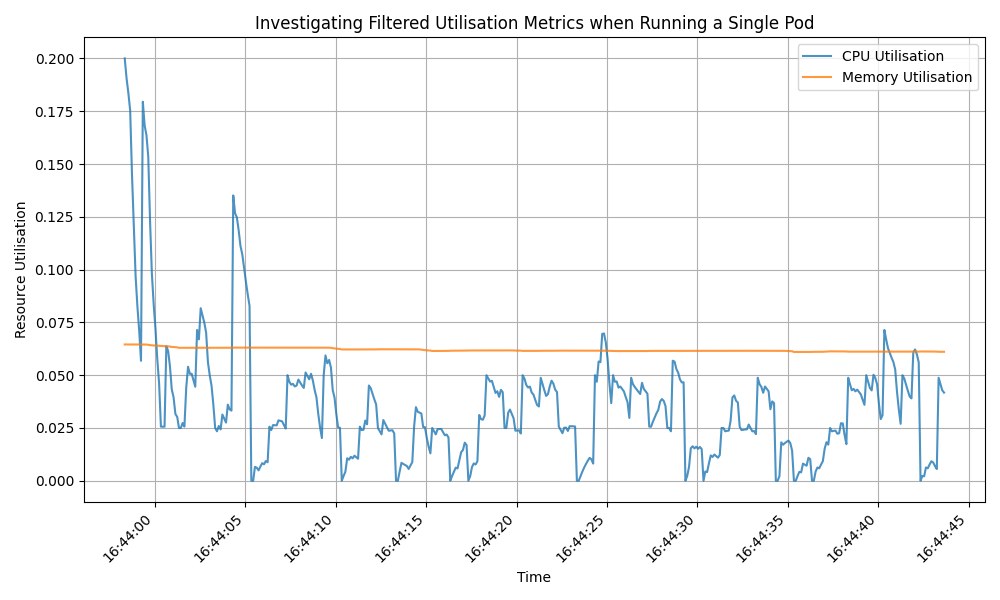
\includegraphics[width=0.45\textwidth]{images/filter-utilisation-baseline.png}
    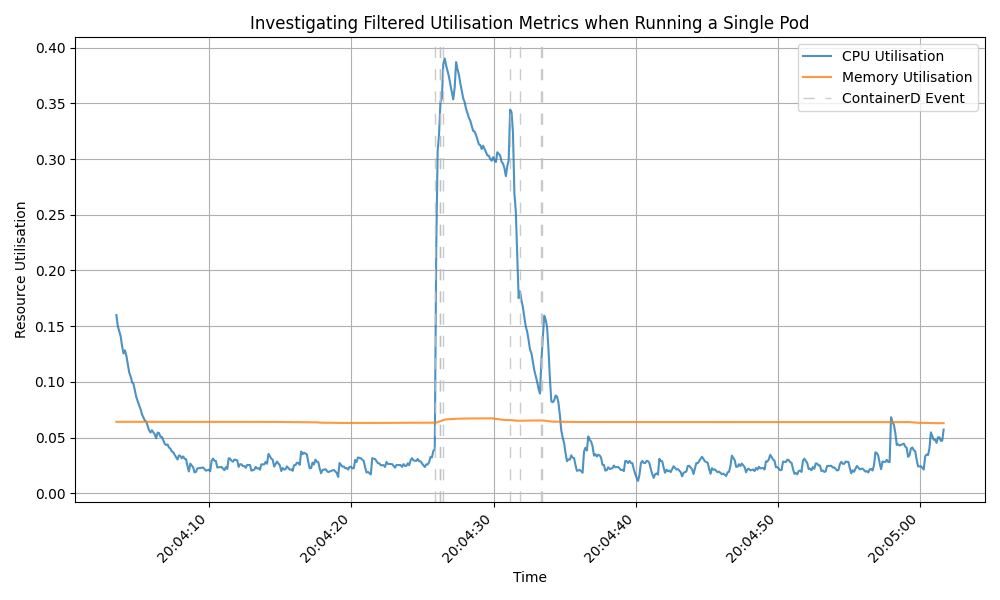
\includegraphics[width=0.45\textwidth]{images/filter-utilisation-single.png} \\
    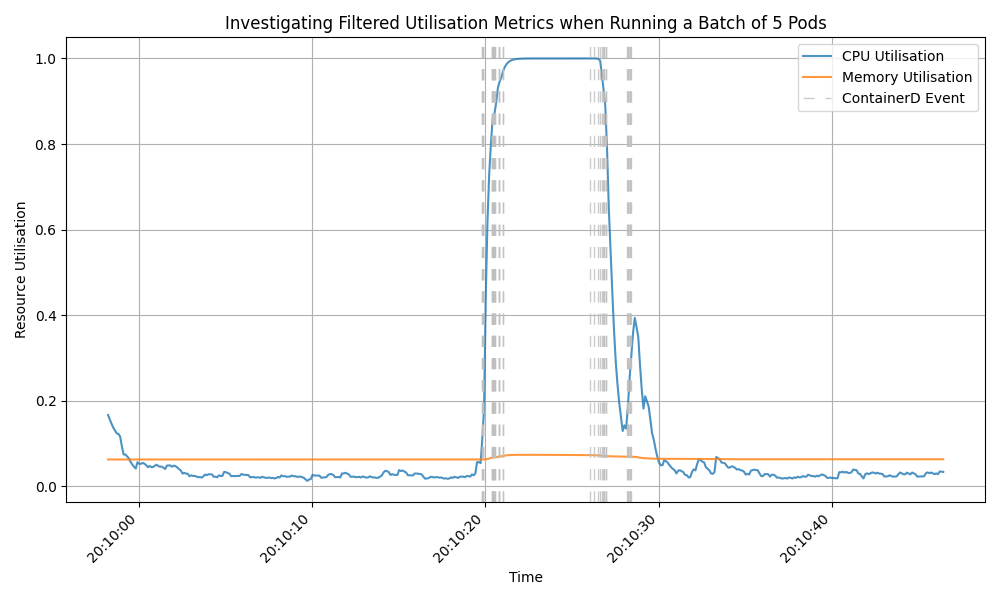
\includegraphics[width=0.45\textwidth]{images/filter-utilisation-smallbatch.png}
    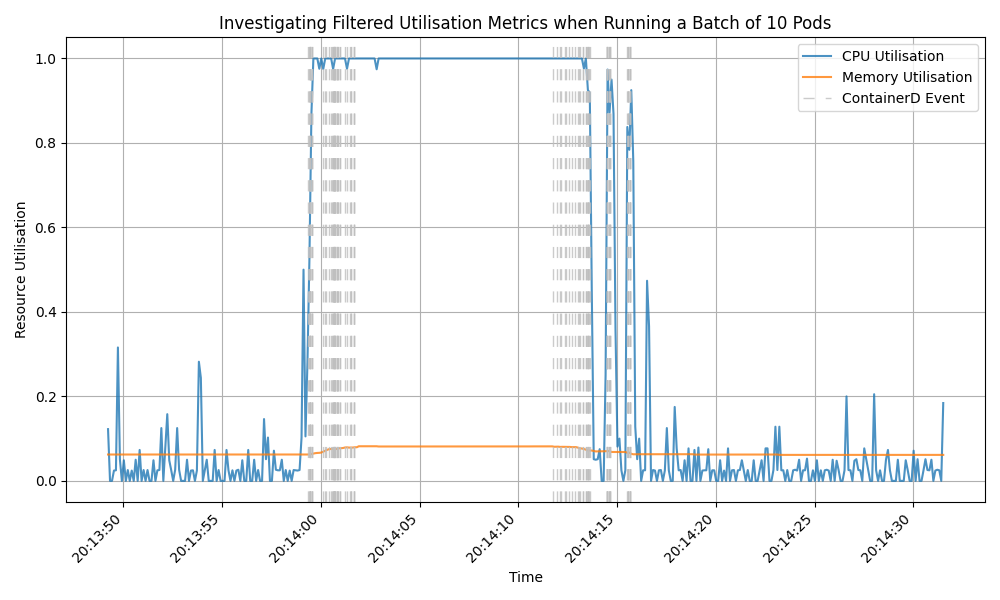
\includegraphics[width=0.45\textwidth]{images/filter-utilisation-bigbatch.png}
    \caption{This figures shows the smoothed metrics under different workloads.}
    \label{fig:filtered-metrics-eval}
\end{figure}

Comparing Figure \ref{fig:utilisation-eval} with \ref{fig:filtered-metrics-eval}
demonstrates the dampening of the Dynamic EMA and its quick responsive to
prolonged changes in workloads. While more sophisticated filters exist, they
were not considered due to their higher computational cost and thus would rob
scheduled pods of the available resources. I had considered applying the filter
directly to the signal instead of the collected telemetry, but by only filtering
the signal, it would allow the local model to be polluted by these
container-event resource spikes.

\subsection{Signal Generation}
In the Spazio Pod, the signal is calculated at a frequency of 1Hz. This
frequency is the same frequency at which the local model is updated. This
ensures that the signal tracks with the local model. Increasing the frequency
would give the central scheduler a more up-to-date view of a Node's resource
status, but would incurr additional resource overhead. Not only would this
overhead reduce the available resources to other Pods, it would be reflected by
a lower signal, potentially reducing capacity a Node advertises.

To check for a correct implementation of the signal, I measured the calculated
signal when under the situations described in \ref{sec:capacity-signal}. The
collected measuremets are shown in figures \ref{fig:signal-evaluation-cpu} and
\ref{fig:signal-evaluation-mem}

\begin{figure}[H]
    \centering
    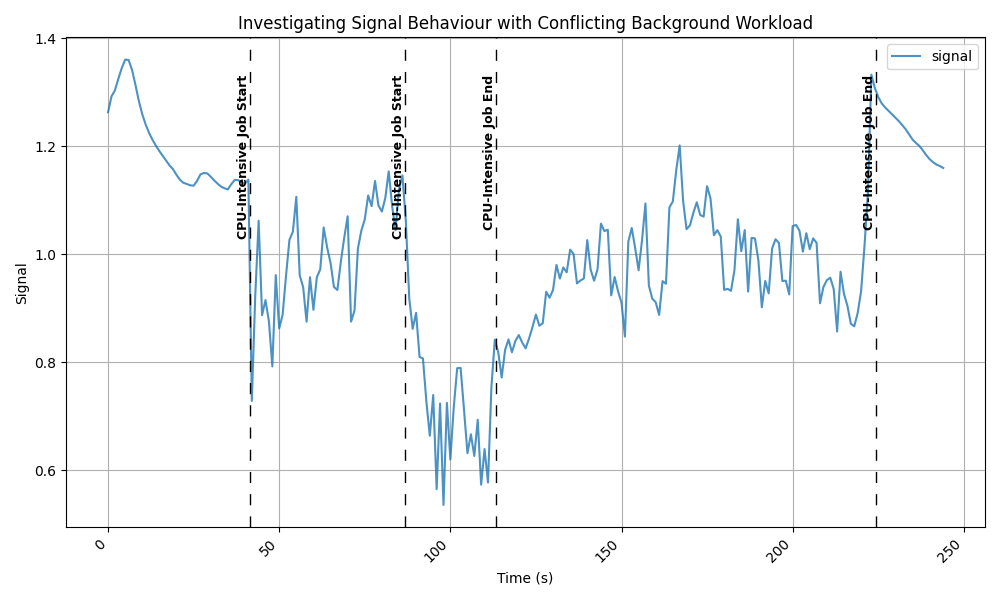
\includegraphics[width=\textwidth]{images/signal-with-cpu.png}
    \caption{The calculated capacity signal of a Node running \texttt{ng-stress
    --cpu=8 --cpu-load=25}. While running this workload, $1000$ Pods running
    \texttt{bpi(2000)} was scheduled across surrounding Nodes.}
    \label{fig:signal-evaluation-cpu}
\end{figure}
\begin{figure}[H]
    \centering
    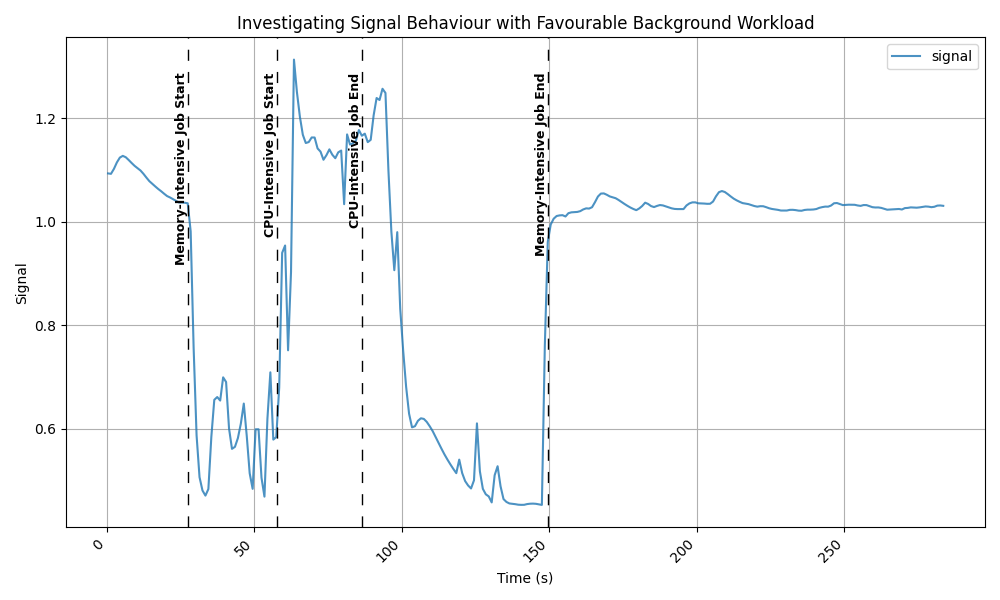
\includegraphics[width=\textwidth]{images/signal-with-memory.png}
    \caption{The calculated capacity signal of a Node running \texttt{ng-stress
    --vm=4 --vm-bytes=4G}. While running this workload, $1000$ Pods running
    \texttt{bpi(2000)} was scheduled across surrounding Nodes.}
    \label{fig:signal-evaluation-mem}
\end{figure}

Figures \ref{fig:signal-evaluation-cpu} and \ref{fig:signal-evaluation-mem}
demonstrates how a Node's capacity signal reacts to changes in surrounding
workloads when experiencing different resource usage. In Figure
\ref{fig:signal-evaluation-cpu}, the measured Node is running a light CPU-focused
workload. Once the CPU-intense workload is scheduled on surrounding Nodes, the
measured Node's capacity signal drops. This is expected as the local models of
surrounding Nodes will reflect a more costly CPU-focused workload. As a result,
when the measured Node aggregates its local model, its new model will reflect
this higher CPU usage with a larger $\sigma_1$ value. As the measured Node's
directions of the measured Node's resource usage and expected workload are still
CPU-focused, the increased $\sigma_1$ value results in a lower $k$, and thus a
lower capacity signal.

In Figure \ref{fig:signal-evaluation-cpu}, the measured Node is running a light
Memory-focused workload. When the CPU-intense workload is scheduled on surrounding
Nodes, the measured Node's capacity signal increases. This matches
\ref{sec:capacity-signal} hypothesis. Like in the previous scenario, the global model
reflects a heavy CPU-focused workload, and thus, so will the aggregated local
model of the measured Node. However, as the measured Node's resource usage is
now orthogonal to the expected resource usage, a larger constant $k$ is needed
to maximise a resource. This reflects the sharp increase in capacity signal we
observe in figure \ref{fig:signal-evaluation-mem}.

\subsection{Calculating Cost and Capacity}
As the new proposed signal also used its current resource usage in the
calculation, pods scheduled on a node would not impact the signal until they had
started running. Thus, I needed a means of reserving the signal to prevent the
scheduler from running away and greedily assigning all pods to the node with
highest score. As pod workload may vary over time, I needed a means of
dynamically estimating the "signal cost" of assigning a pod to a node. In
addition, I needed the method to be able to handle multiple pods being created
and deleted at once.

\subsubsection{Detecting Pod Events}
There are numerous ways to detect the addition and removal of pods from a node.
I investigated two: watching the Kubernetes API and watching the ContainerD
events. The goals of the listeners were as follows:
\begin{itemize}
    \item Detect the creation and deletion of pods to establish a pod count
    \item Provide warning for potential container-caused churn
\end{itemize}
The latter requirement is needed as the Dynamic EMA used on the resources won't
be able to smooth longer resource spikes caused by a burst of multiple container
events. Instead, by detecting pod events earlier, we can halt capacity and
per-Pod cost estimations until the burst has passed.

\begin{figure}[H]
    \centering
    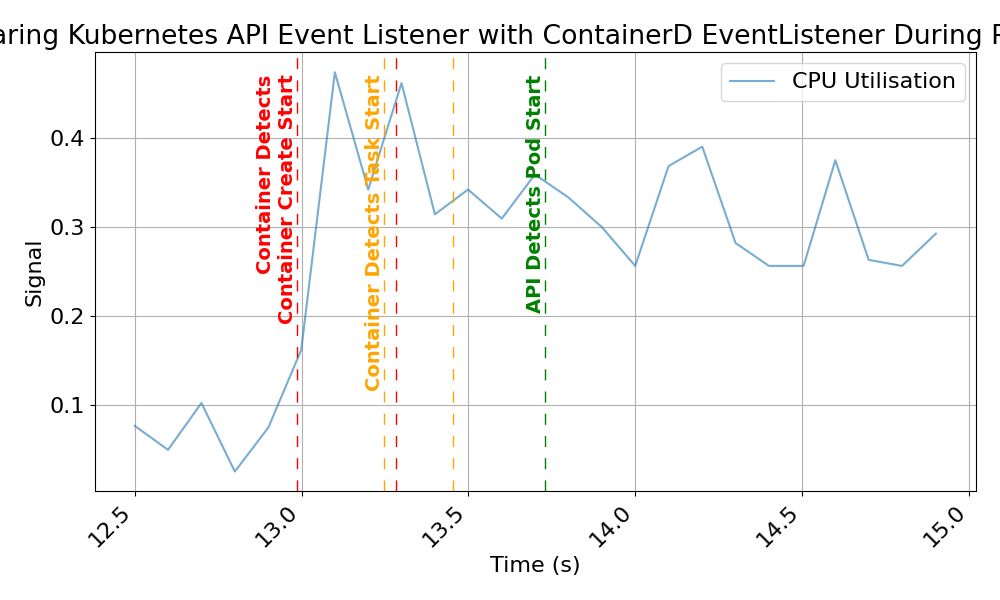
\includegraphics[width=\textwidth]{images/event-comparison-start.png}
    \caption{When different event listeners detected the creation of a Pod.}
    \label{fig:event-evaluation-start}
\end{figure}

\begin{figure}[H]
    \centering
    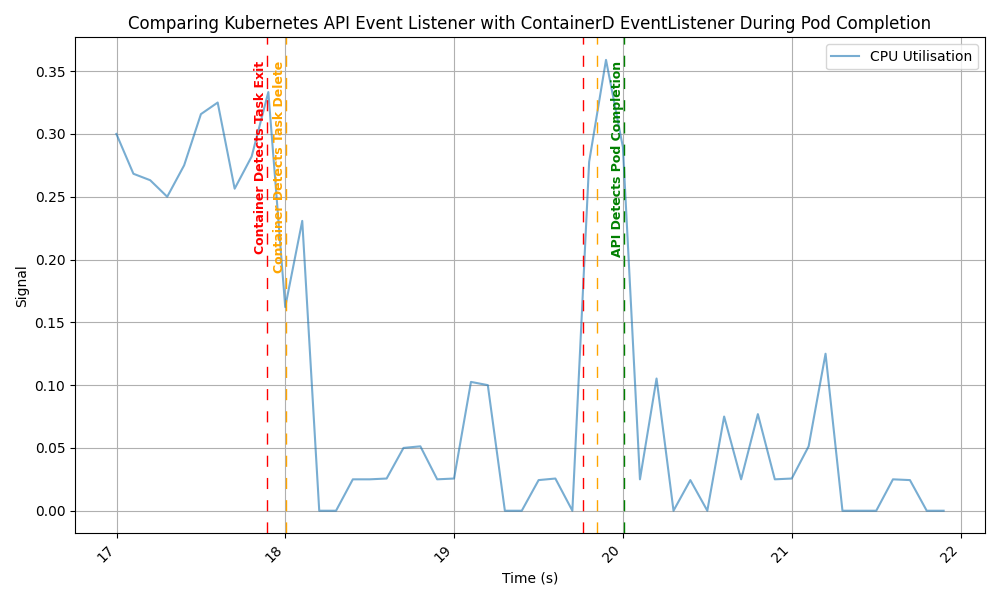
\includegraphics[width=\textwidth]{images/event-comparison-end.png}
    \caption{When different event listeners detected the completion of a Pod.}
    \label{fig:event-evaluation-end}
\end{figure}

As shown in figures \ref{fig:event-evaluation-start} and
\ref{fig:event-evaluation-end}, the two-way latency from sending events
to the \verb|kube-apiserver| before then detecting results in the Kubernetes API
listener to miss the spikes caused by container events. Without a forewarn, nodes
will include container event resource spikes into their resource predictions. On
the other hand, we can see that certain container events precede the spikes.
While handling container events is more complex, it can alert the node of
potential spikes and thus reduce the introduction of noise into our
calculations.

\subsubsection{Estimating Pod-Cost}
As mentioned in Section \ref{sec:spazio-cost-capacity}, Spazio assumes a Node
has the capability of estimating its capacity and per-Pod cost. I needed a
streaming signal processing technique with a low-overhead and the ability to
work with a dynamic system (handle changes in workloads over time). A Kalman filter
\cite{} is a powerful algorithm used for estimating the true state of a dynamic
from a series of noisy and uncertain measurements. It's widely applied in fields
like navigation (GPS), robotics, signal processing and control systems.

TODO: Should I explain what a Kalman filter is in more detail?
I devised three Kalman filter-based approaches to estimating reservation costs.
\begin{itemize}
    \item 1D Kalman Filter predicting reservation cost based on the function:
        \[\Delta \text{signal} = \Delta \text{no. of running pods} \times
        \text{cost}\]
    \item 2D Kalman Filter to predict the signal based on the function:
        \[\text{signal} = \text{capacity} + \text{per pod cost} \times \text{no.
        of pods}\]
    \item Two separate 1D Kalman Filters predicting the equation:
        \[\text{signal} = \text{capacity} + \text{per pod cost} \times \text{no.
        of pods}\].
        This dual filter approach has each filter learn a separate variable. By
        splitting the filter into two, it prevents non-zero covariance
        entries in the $P$ matrix which cause the oscillations seen in the 2D
        Kalman filter.
\end{itemize}
To smooth out predictions, I employed two techniques. The first technique
utilised the container event listener: on detection of container churn, the
Spazio Pod would temporarily halt estimations until it had passed. Secondly, I
halted estimates once the signal reached 0. When the capacity signal is 0, it
indicates that at least one resource is at capacity. If this occurs and another
Pod begins running on the same Node, the signal still outputs 0. Without halting
estimates, the filters would continue to decrease the per-Pod cost, resulting in
an inaccurately low per-Pod cost and thus advertise too large of a capacity.

\begin{figure}[H]
    \centering
    % 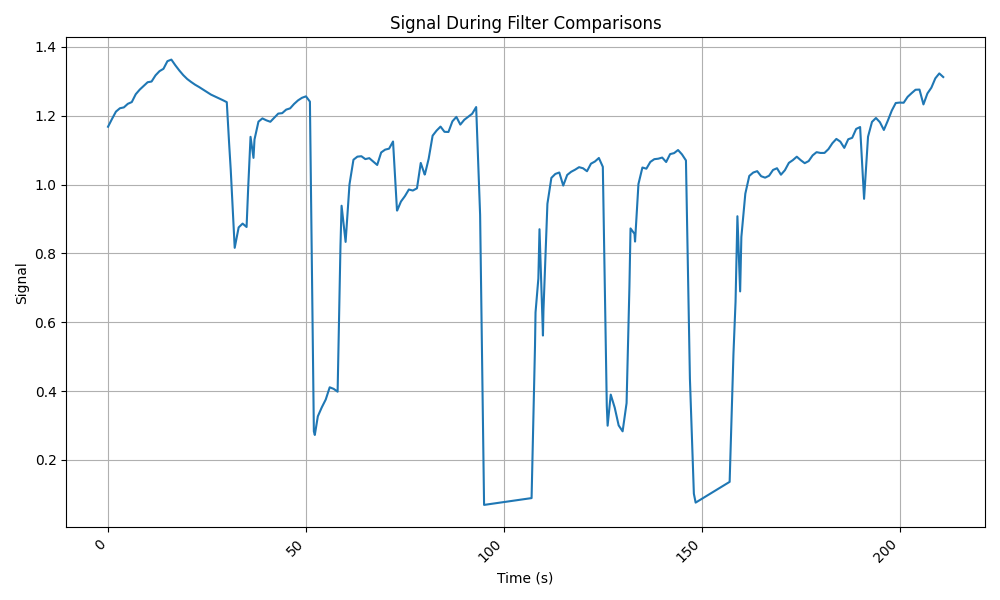
\includegraphics[width=0.45\textwidth]{images/filter-signal.png}
    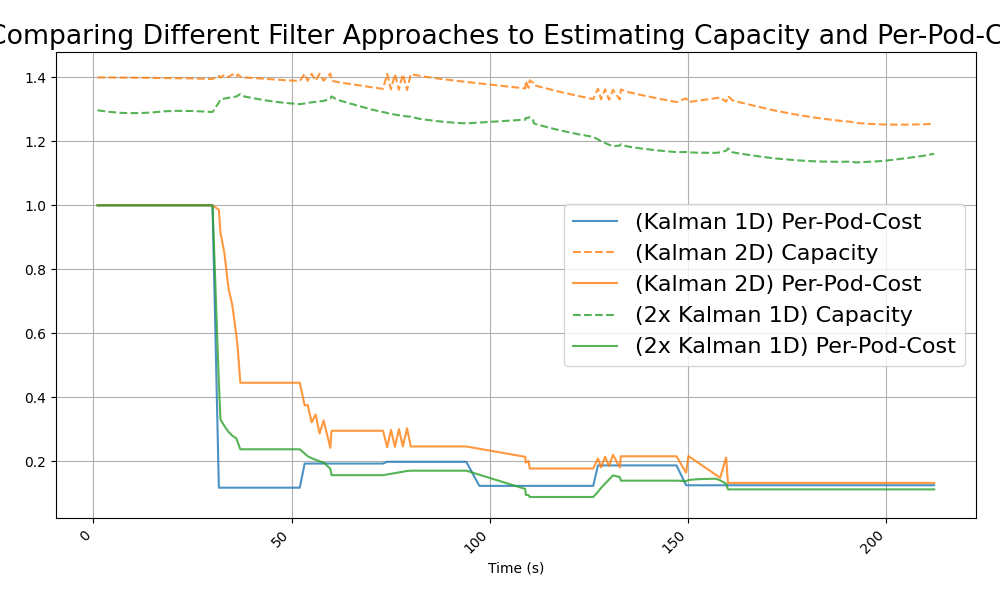
\includegraphics[width=\textwidth]{images/filter-comparison.png}
    \caption{The estimates of the Kalman filters when Node experiences
    variable-sized bursts of \texttt{bpi(2000)} Pods.}
    \label{fig:filter-evaluation}
\end{figure}
To decide the optimal approach, I observed each methods' behaviour when
executing Jobs of various sizes. This is depicted in Figure
\ref{fig:filter-evaluation}.
While $\Delta$-based Kalman filter produced accurate estimates of per-Pod cost,
its one-dimensional property prevents it from estimating the capacity of the
Node. However, its stability inspired the double Kalman filter approach.
The 2D Kalman filter approach provides a simple method for estimating both the
Node's capacity and its per-Pod cost. However, to ensure faster convergence, I
used large constants in the $Q$ matrix. This resulted in large oscillations
as the filter attempts to correct any error by modifying both the capacity and
cost variables. Finally, the dual Kalman filters approach converged quickly on
an accurate estimation without exhibiting the oscillations seens in the 2D
Kalman filter. This made the Dual 1D Kalman filter the optimal choice.

\section{Aggregation Server}
\begin{figure}[H]
    \centering
    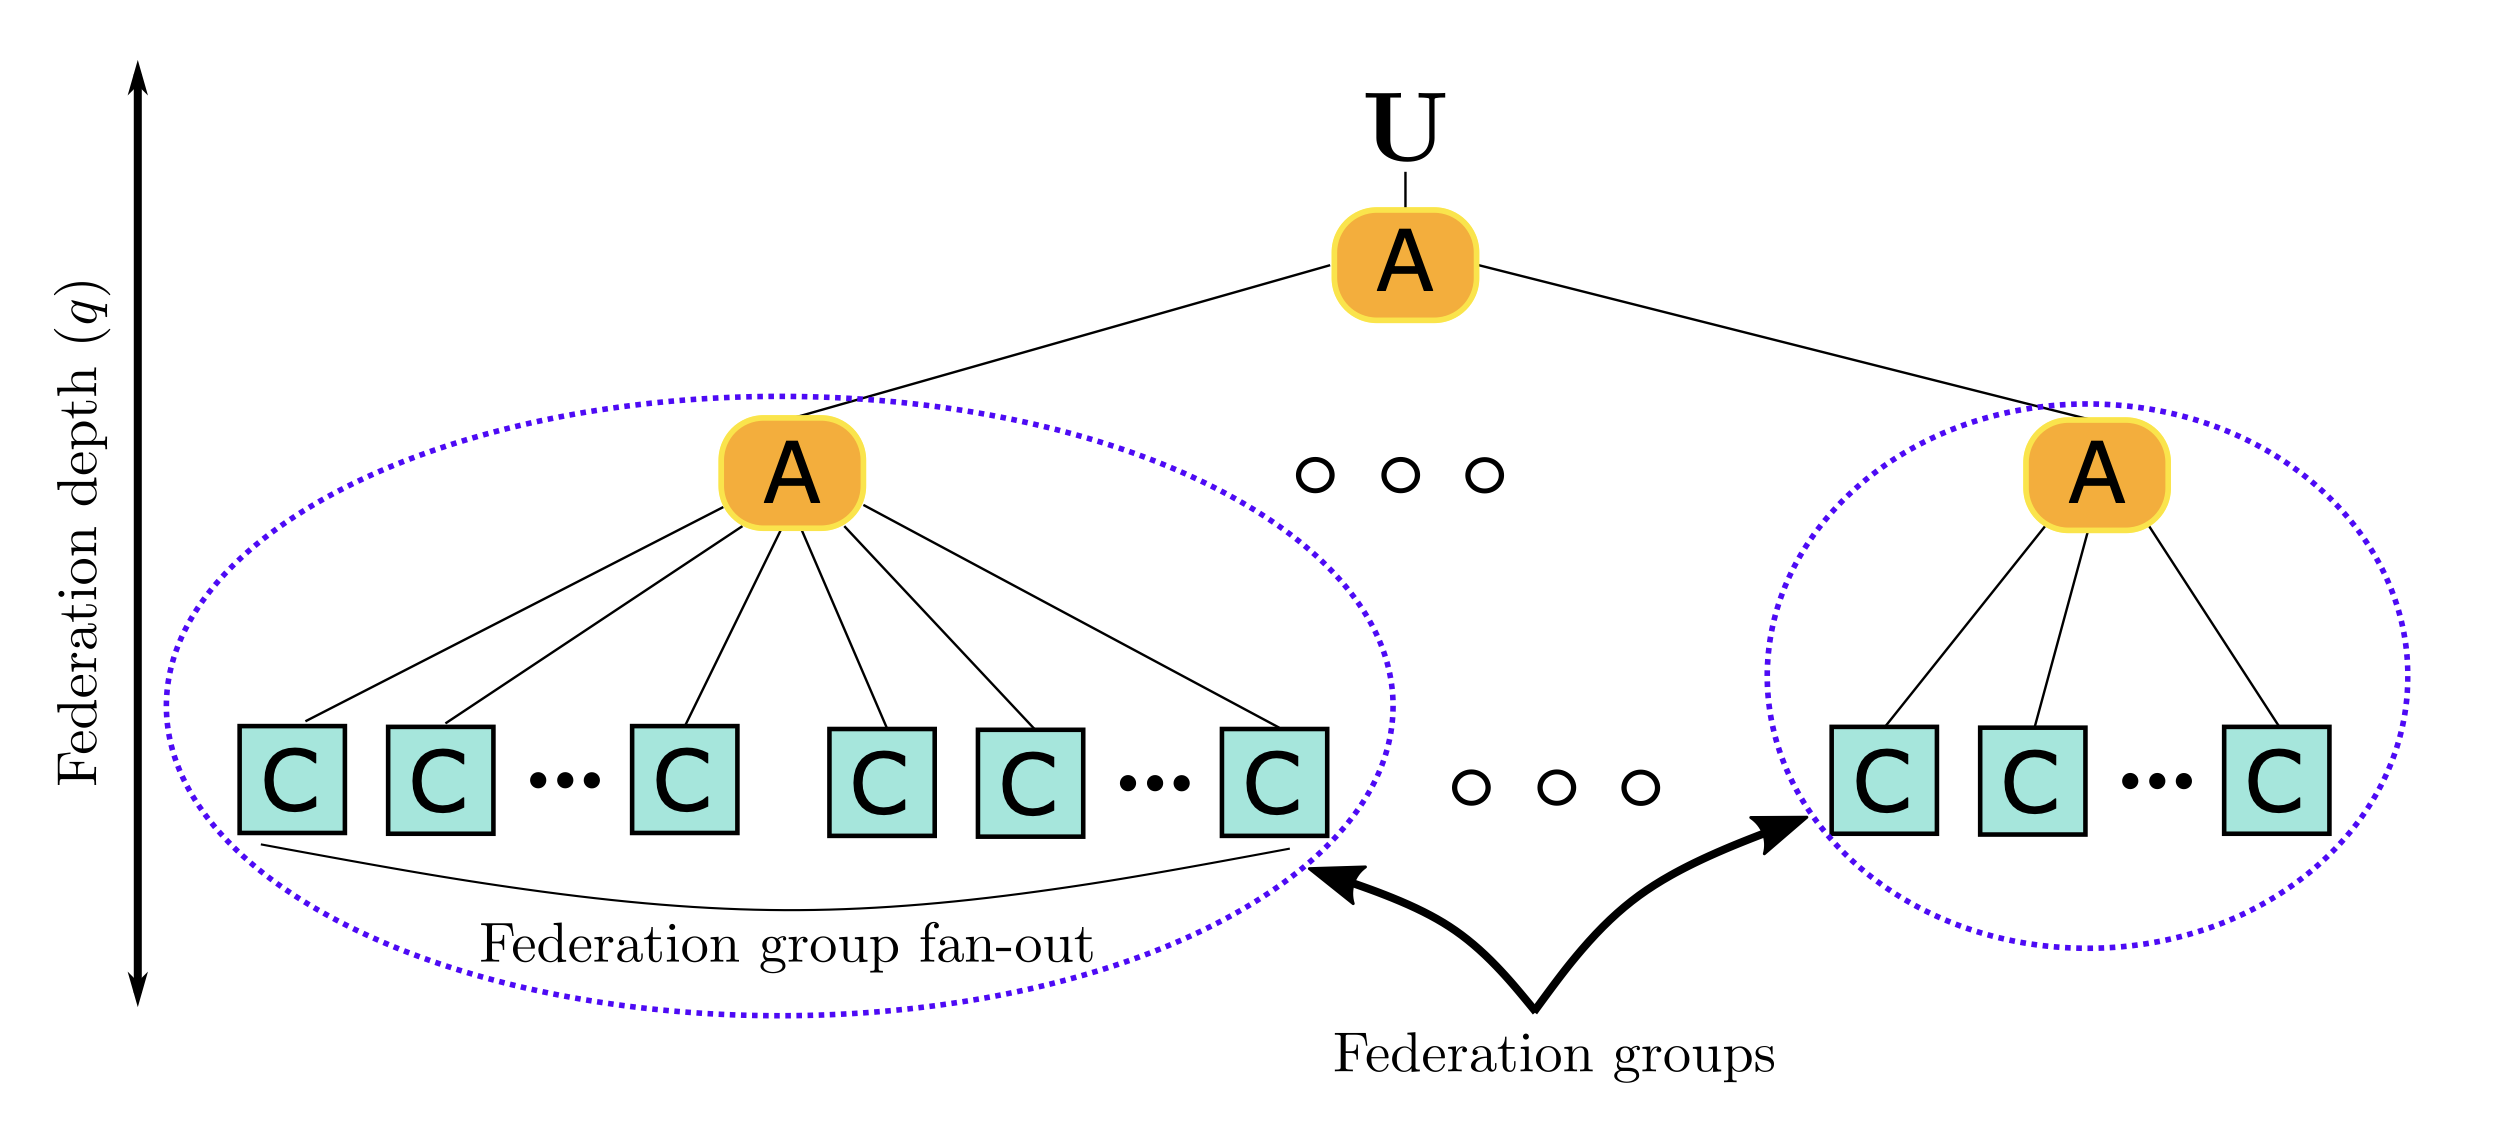
\includegraphics[width=\textwidth]{images/pronto-agg.png}
    \caption{How local models are aggregated in Pronto. Dedicated aggregator
    nodes propagate the updated subspaces until the root is reached.}
    \label{pronto-agg}
\end{figure}
Pronto aggregation approach is similar to the distributed agglomerative summary
model (DASM) \cite{}. Local models are aggregated in a "bottom-up" approach
following a tree-structure depicted in Figure \ref{pronto-agg}. While the
this approach is stated to required minimal synchonisation, it requires
mutliple dedicated Pods and Kubernetes inherent communication latency could
result in a significant latency between a change in workload and the global
model reflecting the change.

Therefore, I decided to use a flat on-the-fly approach to aggregation: when the
Aggregation Server receives an aggregation request with a Node's local model,
rather than aggregating the model before returning the result, the server
enqueues the model to be aggregated and returns its latest view of the
aggregated model. This implementation trades consistency for latency.


The Aggregation Server Pod
\begin{figure}[H]
    \centering
    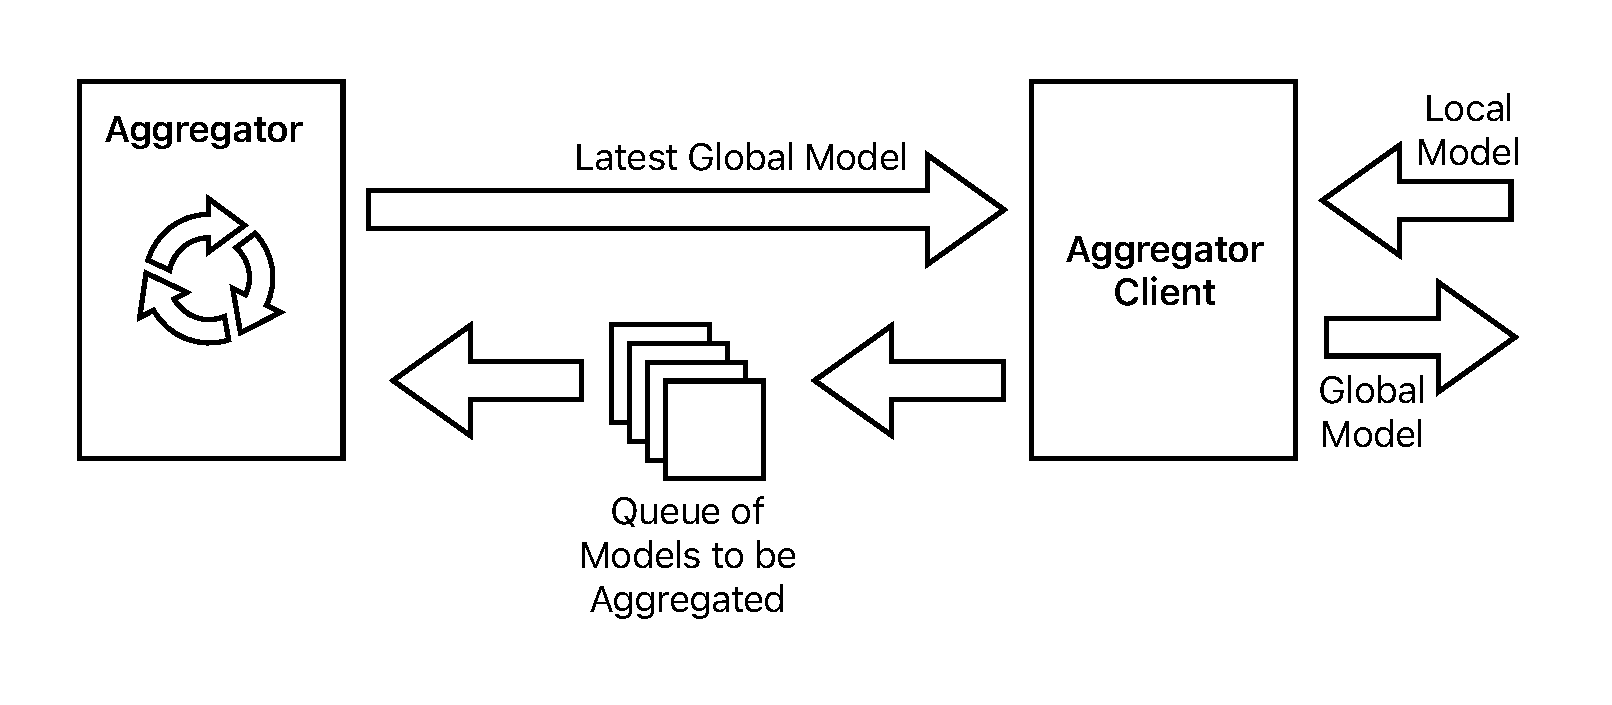
\includegraphics[width=\textwidth]{images/spazio-agg.pdf}
    \caption{Core components within the aggregator pod}
    \label{spazio-agg-components}
\end{figure}

As mentioned earlier in section \ref{}, the aggregator trades
. On aggregation request it returns the
latest global model and enqueues the local model it received. Another worker
thread running in the background dequeues local models and merges them into the
global model.

Explain why I use a flat style aggregation rather than a hierarchical design.
Core idea is the choice of efficiency and lateny vs consistency.

The aggregation of local models to produce a global model also uses the same
iterative-SVD as defined in section \ref{sec:local-model-construction}. In
addition, instead of using a hierarchical aggregation system, I use flat
aggregation service - all aggregation requests are handled by a single node.
In the original Pronto paper, the authors assumed that there was no
communication latency. However, in a real-world cluster this assumption does not
hold. Adding additional aggregation layers would increase the overall aggregation
latency.

Instead with a aggregation server, I can reduce the overall latency of
aggregation requests. To reduce request latency further, actual model
aggregation is not performed on the request's critical path. On receipt, the local
model is enqueued to be aggregated and the latest global model is returned. A
background thread iterative-SVD merges the queued local models into the global
model. In summary, this system trades consistency for latency and throughput,
which becomes a dominant factor when scaling to hundreds of nodes.

\section{Scheduler Pod}
\begin{figure}[H]
    \centering
    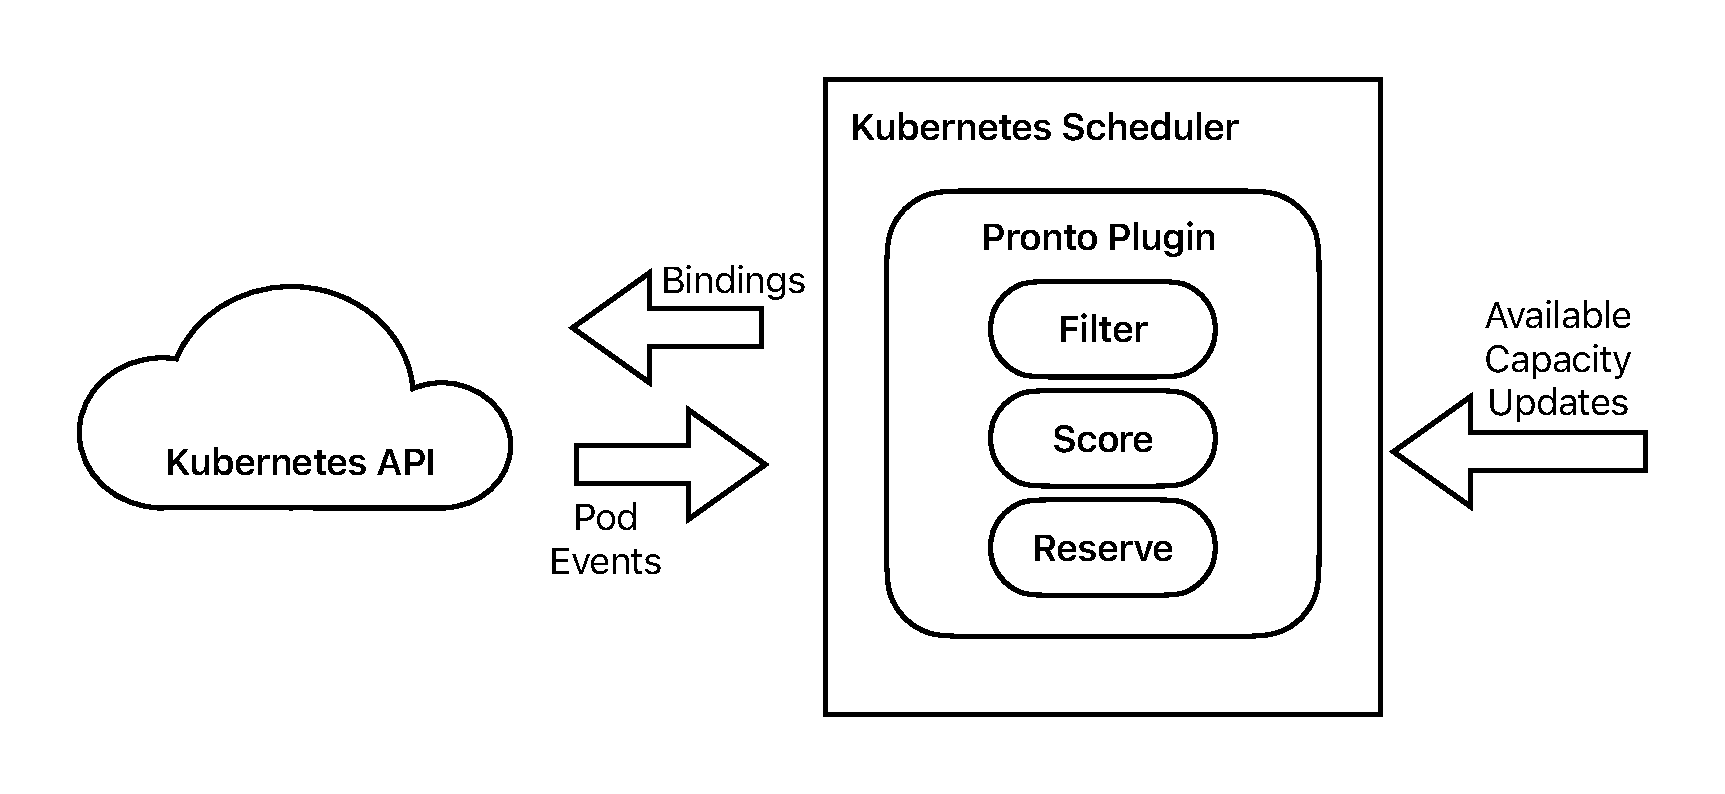
\includegraphics[width=\textwidth]{images/spazio-sched.pdf}
    \caption{Core components within the central scheduler pod}
    \label{spazio-sched-components}
\end{figure}

\subsection{Kubernetes Scheduler Plugin}
This section gives the motivation for using a Kubernetes Plugin. Core Ideas:
ease of use, access to efficient data structures.

I decided to implement the scheduling component as a Kubernetes Framework
Plugin. The standard Kubernetes scheduler exposes a series of extension points,
which allows users to define custom functions within the scheduling cycle. A
Scheduler Plugin is a more favourable approach as it allows me to use an
existing system designed to operate at an industrial level. The Pronto Plugin
implements the following extension points:
\begin{itemize}
    \item: Filter - this function filters out any nodes based on $
        \text{capacity available} - \text{capacity reserved} < \epsilon$.
    \item Score - this function assigns a score based on the available capacity.
        The greater the available capacity, the greater the score and thus the
        more likely it is to be chosen for pod placement
    \item Reserve - once a node is chosen to host the pod, the reserve function
        records the pod's name and increments the node's reserved capacity.
\end{itemize}

This pod also has a Kubernetes API Pod Event listener which listens out for pods
that have transitioned from the Pending status. For each event that this occurs,
it checks if this pod was scheduled by the scheduler and decrements its value
from reserved.


\subsection{Filter}
This section explains the Filter function

\subsection{Score}
This section explains the Score function

\subsection{Reserve}
This section explains the Reserve function
